\section{Model Exercise 1-2 (06): Shrinkage of clay}
\label{sec:mex06}
%------------------------------------------------------------------------------
\Authors{Amir Sattari et al.}
%------------------------------------------------------------------------------
The shrinkage process and developed micro structure pathways in Opalinus clay stone is the focus of the this model exercise (MEX 1-2).The surface and whole body cracking under shrinkage will be investigated and numerical simulations will be used to not only simulate the fracking pattern but also to determine the change of hydraulic conductivity during shrinkage. 
%------------------------------------------------------------------------------
\subsection{Experimental set-up}
%------------------------------------------------------------------------------
The prepared two cylindrical thin sections of sandy Opalinus claystone \ref{fig:Amir_ME6_Sample} (Mont-Terri) with dimension of 100x10 mm (DxH) are located inside the desiccator \ref{fig:Amir_ME6_Full_Setup} with the constant room temperature of 20\ °C. On the surface of the first sample two linear strain gauge sensors in perpendicular and parallel to the layering of the bedding are installed \ref{fig:Amir_ME6_Sensors} and finally covered with the adhesive to protect the sensor from environmental temperature and humidity changes \ref{fig:Amir_ME6_Sensors_Final}. The second sample is used to determine the water content change under different applied osmotic suction values. The considered saturated salt solutions \cite{Minardietal2016} as well as their resulted suction values are listed in \ref{table:Amir_ME6_SaltSolutions}.

\begin{figure}[!ht]
\begin{subfigure}[c]{0.48\textwidth}
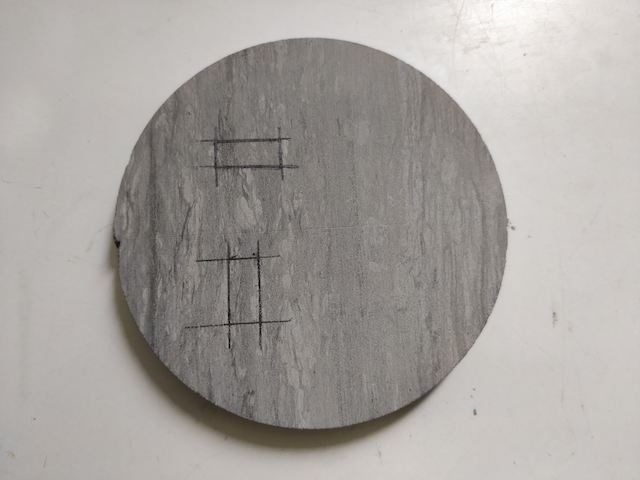
\includegraphics[width=1\textwidth]{figures/Amir_ME6_Sample.png}
\subcaption{The thin cylindrical Opalinus claystone sample}
\label{fig:Amir_ME6_Sample}
\end{subfigure}
\hfill
\begin{subfigure}[c]{0.48\textwidth}
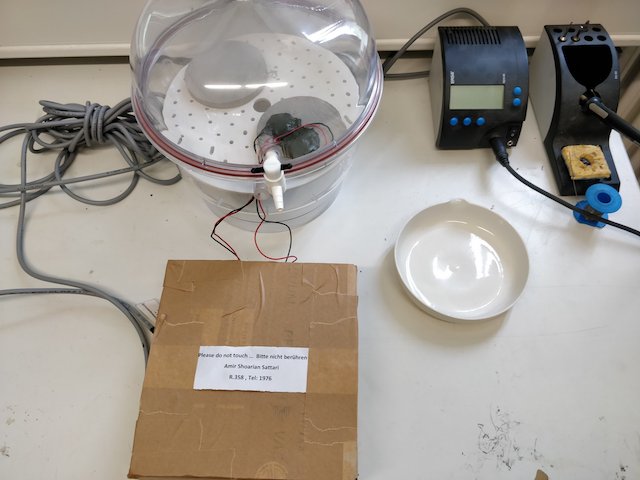
\includegraphics[width=1\textwidth]{figures/Amir_ME6_Full_Setup.png}
\subcaption{The prepared setup with desiccator and strain gauge sensors}
\label{fig:Amir_ME6_Full_Setup}
\end{subfigure}
\caption{The shrinkage and swelling test Procedure}
\end{figure}

\begin{figure}[!ht]
\begin{subfigure}[c]{0.48\textwidth}
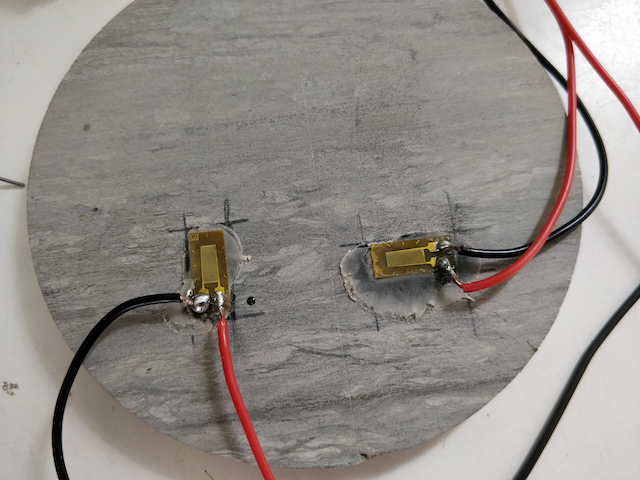
\includegraphics[width=1\textwidth]{figures/Amir_ME6_Sensors.png}
\subcaption{The perpendicular and parallel strain gauges}
\label{fig: Amir_ME6_Sensors}
\end{subfigure}
\hfill
\begin{subfigure}[c]{0.48\textwidth}
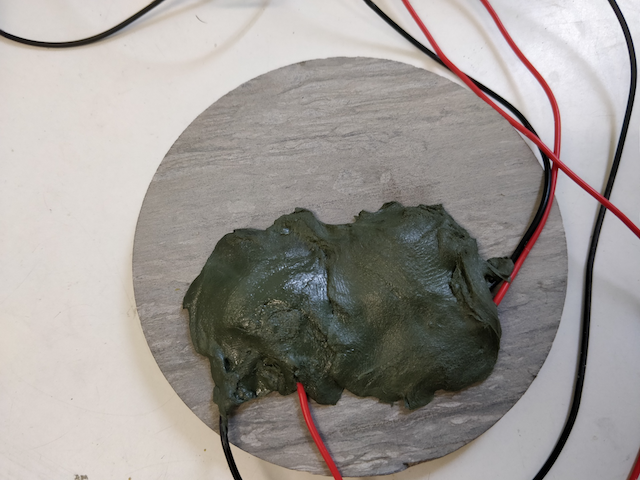
\includegraphics[width=1\textwidth]{figures/Amir_ME6_Sensors_Final.png}
\subcaption{The covering glue for protecting the strain gauges}
\label{fig:Amir_ME6_Sensors_Final}
\end{subfigure}
\caption{The installation of linear strain gauges}
\end{figure}

\begin{table}[h!]
\centering
\begin{center}
\begin{tabular}{ | m{5em} || m{5em}| m{5em} | m{5em} | m{5em} | m{5em} |} 
\hline
Salt Solution & Potassium Nitrate & Potassium Chloride & Sodium Chloride & Magnesium Nitrate & Magnesium Chloride  \\
\hline
 Suction (MPa)  & 9.8 & 22.6 & 39 & 86 & 139   \\ 
\hline
\end{tabular}
\end{center}
\caption{The variation of considered salt solutions}
\label{table:Amir_ME6_SaltSolutions}
\end{table}

The change of strain gauges values with different salt solutions are recorded, where for each salt solution the process stopped when an equilibrium of weight and strain changes are reached. The \ref{fig:Amir_ME6_Experimental_Strain} depicts the change of strain values in parallel and perpendicular directions to the bedding layers. In drying process, in average, the strain sensors perpendicular to the layering depict almost 3.6 times higher values than strain gauges parallel to the layering. 

\begin{figure}[!ht]
\centering
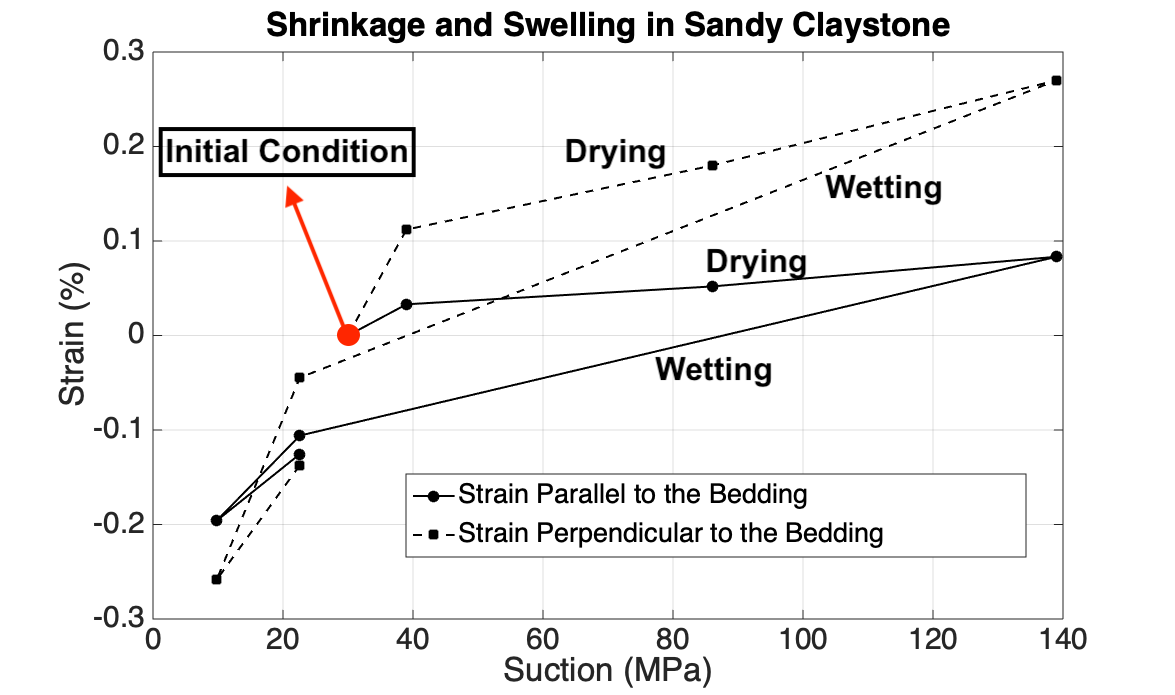
\includegraphics[width=0.75\textwidth]{figures/Amir_ME6_Experimental_Strain.png}
\caption{The Strain Vs. Suction Relation}
\label{fig:Amir_ME6_Experimental_Strain}
\end{figure}

%------------------------------------------------------------------------------
\subsection{Model approaches}

The simulation results from each of the model methods, discrete element method (DEM), lattice element method (LEM) and phase field method (PFM) are described and the accuracy of numerical results for modeling the shrinkage process with change of linear or volumetric strains as well as the change of anisotropic hydraulic conductivity are investigated. 

\subsubsection*{Discrete-Element-Model (DEM)}
\todo{[IfG] Contribution planned?}

\subsubsection*{Lattice element model}
With the application of the dual lattice element \ref{Section:HMLattice}, the hydraulic flow in the domain is simulated. The mechanical lattice element with the integrated interface element \cite{Sattarietal2019b} is implemented to simulate the shrinkage process and fracking in claystone \ref{fig:Amir_ME6_Lattice_Model}. The linear axial strain of the elements according to the \ref{fig:Amir_ME6_Experimental_Strain} is considered to simulate the fracking and hydraulic property changes. 

\begin{figure}[!ht]
\centering
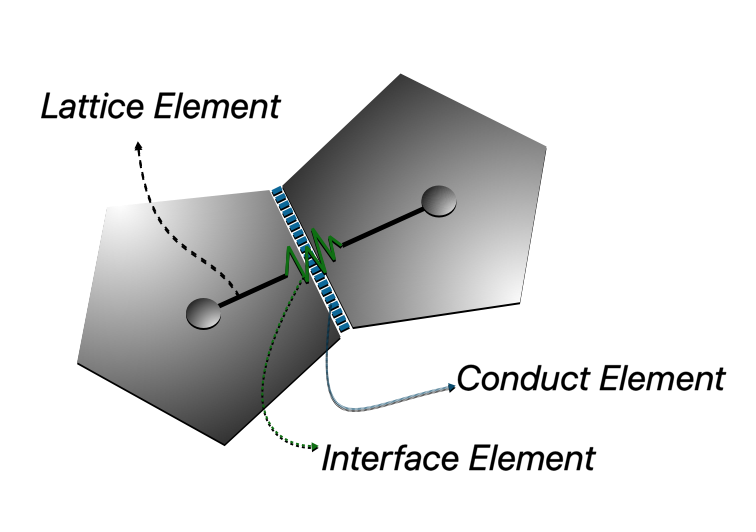
\includegraphics[width=0.75\textwidth]{figures/Amir_ME6_Lattice_Model.png}
\caption{The implemented dual lattice as well as integrated interface element}
\label{fig:Amir_ME6_Lattice_Model}
\end{figure} 

The initial condition values for anisotropic hydraulic conductivity are approximated according to technical Report, Mont Terri 2008-04 as:

\begin{align}
\label{eq:LEM_ME6_1}
\begin{split}
K_\parallel=2\times{10}{^{-13}}\\
K_\bot=0.6\times{10}{^{-13}}
\end{split}
\end{align}

While considering the cubic law for flow transfer through porous medium, the hydraulic aperture and length of interface element is :
\begin{align}
\label{eq:LEM_ME6_2}
\begin{split}
e=\sqrt(K\times12\times\upsilon/g)\\
e_\parallel=4.95\times{10}{^{-10}}\\ e_\bot=2.71\times{10}{^{-10}}
\end{split}
\end{align}

where $\upsilon=1.004\times{10}{^{-6}}$ and g=9.8. 

The vectorizable lattice element with defined layering bedding \ref{fig:Amir_ME6_Lattice_Setup} is used to generate the domain. The interface length is defined based on \ref{eq:LEM_ME6_2}.

\begin{figure}[!ht]
\centering
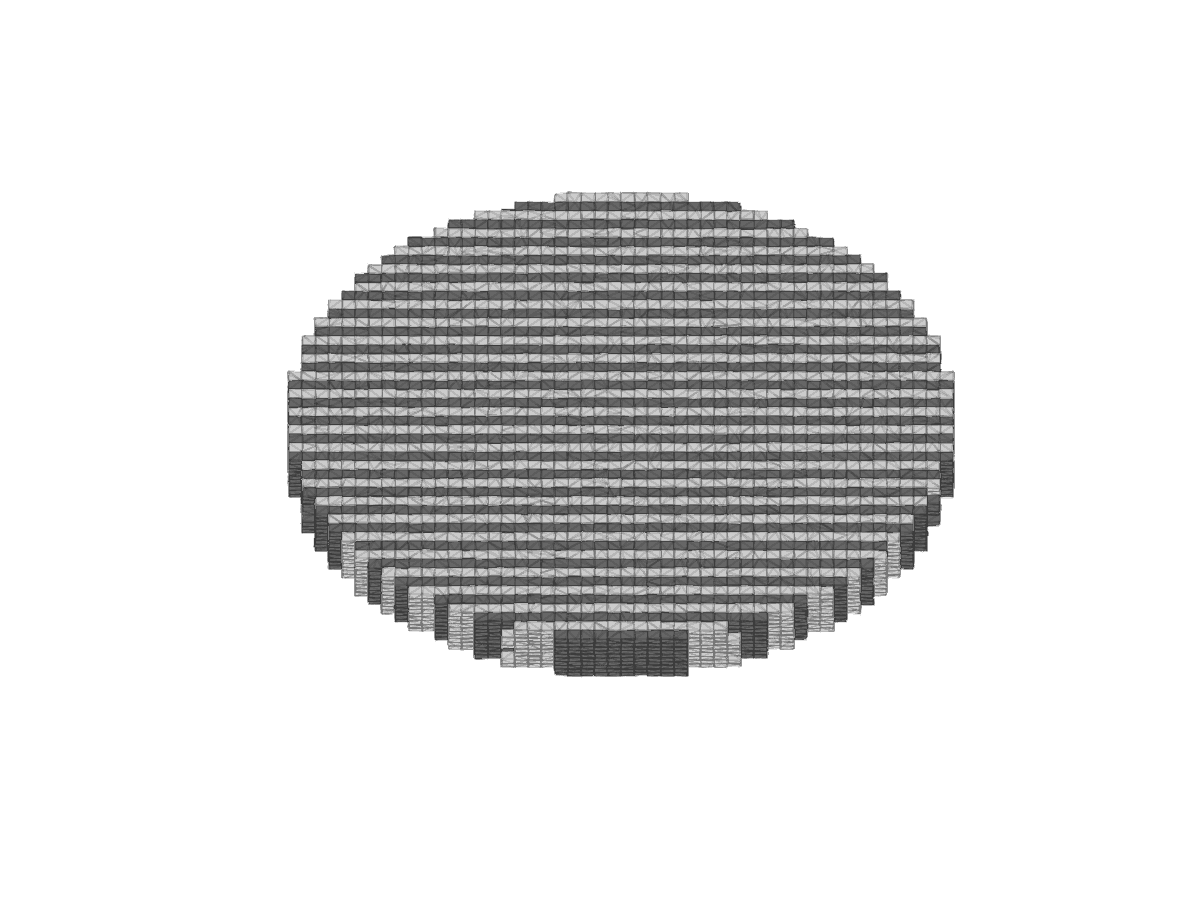
\includegraphics[width=0.75\textwidth]{figures/Amir_ME6_Lattice_Setup.png}
\caption{The generated domain for shrinkage process}
\label{fig:Amir_ME6_Lattice_Setup}
\end{figure} 

\subsubsection*{Finite-Element-Method: Variational-Phase-Field (VPF)}
\todo{[UFZ] Contribution planned?}
FEM mesh~\ref{fig:ME5_VPF_setup}.

\begin{figure}[!ht]
\centering
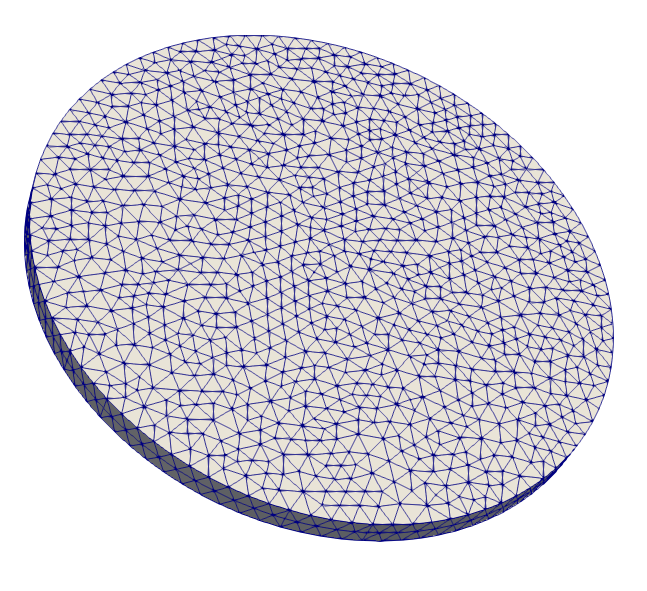
\includegraphics[width=0.75\textwidth]{figures/ME5_VPF_mesh.png}
\caption{The generated FEM mesh for shrinkage process}
\label{fig:ME5_VPF_setup}
\end{figure} 
%------------------------------------------------------------------------------
\subsection{Results and discussion}